%%%%%%%%%%%%%%%%%%%%%%%%%%%%%%%%%%%%%%%%%%%%%%%%%%%%%%%%%%%%%%%%%%%%%%%%%%%%%%%%%%%%%%%%%%
\section{Visualizing Taxonomies and Connectivity Data} \label{sect:visualization}        %
%%%%%%%%%%%%%%%%%%%%%%%%%%%%%%%%%%%%%%%%%%%%%%%%%%%%%%%%%%%%%%%%%%%%%%%%%%%%%%%%%%%%%%%%%%

Treemaps~\cite{JS91} are an effective technique to visualize hierarchical data by using nested shapes in a space-filling layout.
Each shape represents a geometric region, which can be subdivided recursively into smaller regions. The standard shape is a rectangle.
Nodes in a treemap, also called \emph{tiles}, represent individual data items in a dataset. Node size, color and text label can be used to represent attributes of the data item. One-layered treemaps can display data attributes but are not very good at emphasizing the place of an item in the overall hierarchical structure. To compensate for that, a small margin with structural labels is typically used. In treemaps displaying hierarchical structures, it is possible to navigate among different layers and zoom into selected tiles~\cite{BL07}.

% TODO: rewrite the 'flat treemap' text for a bit of extra clarity (MH)

To create a treemap, one must define a tiling algorithm - a way to divide a tile into sub-tiles of specified areas.
Tiling algorithms used for typical applications of treemaps such as e.g., visualization of folders in files in the computer file system with their respected sizes, do not associate tile positions with any characteristic of the data. This is not the case in our scenario: while a user navigates among different layers, filters data and zooms into selected areas, the tiles should be kept in the same relative positions to each other. Otherwise, the user's perception of the displayed information will be quickly disrupted. Moreover, our tiling algorithm should allow the user to enforce constraints on tile positions to make the treemap views structurally resemble body regions. Hence, we developed a stable and customizable tiling algorithm that arranges tiles according to a given template~\cite{KBK14}.

For a set of $n$ data items with no positional constraints, a default template is created that consists of $\lfloor \sqrt{n}\, \rfloor$ rows and $\lceil \sqrt{n}\, \rceil$ columns in each row but the last one (which may contain fewer columns). If the positional data is available (e.g., FMA ontology adjacent-to relation) or a user wants to rearrange the data manually, a custom template is associated with the parent node of the dataset items. The template is a hierarchical structure
$\bigl\{\mathit{splitType}, \{\},\ldots, \{\}\bigr\}$ where $\mathit{splitType} \in \left\{\mathrm{slice}, \mathrm{dice}\right\}$ defines a way to split the rectangle into sub-rectangles: vertically or horizontally. By recursively splitting the available area into sub-rectangles, one can define complex layouts that enforce two dimensional constraints in the form ``$x$ is left/right of $y$'' or ``$x$ is above/below of $y$'' where $x$ and $y$ are individual data items or groups of data items that in their turn can be allocated as needed using the same technique.

The schematic body plans created using template-based treemaps can be seen in \cref{fig:treemaps}. \Cref{fig:24tiles} shows the top level 24 tile body anatomy plan. The choice of this layout is explained by \cref{fig:tilemap-cylinder}, which shows how it can conceptually wrap around the longitudinal axis of the human body. The treemap layout is controlled by the (default) templates and remains stable during navigation.


\subsection{Connectivity data} %%%%%%%%%%%%%%%%%%%%%%%%%%%%%%%%%%%%%%%%%%%%%%%%%%%%%%%%%%%

With the treemap-based body plans as background, we overlay the schematic representation of \emph{body systems} such as circulatory, respiratory, or nervous systems. Body systems are essentially graphs with nodes corresponding to body parts (treemap tiles) or entities inside of body parts (proteins, cells, etc.), and their edges represent organ system compounds such as blood vessels or nervous connections that pass through such body parts or sub-parts.
%%
They may also contain auxiliary nodes that are not represented on the treemap but still carry important biomedical information.

Body systems are intrinsically complex and require efficient data visualization techniques to help avoid clutter induced by the large amount of graph edges and their crossings. To support the GUI functionality, body systems must allow users to overview large parts of the body systems as well as to trace individual connections and analyze their structure. In this context, edge bundling techniques~\cite{Hol06,GHN+11,HET12} have been proposed to improve perception of connectivity data in large dense graphs. Such techniques generally rely on edge rerouting strategies that are either solely targeted at improving visual perception (by using the positions of nodes) or exploit the relationships among connectivity data as guidelines for a more natural allocation of graph edges and nodes. Our application requires a mixture of these techniques.

As an example, consider the schematic visualization of blood vessels in human body. Our initial dataset is a graph based on the FMA resource, and consists of approximately 11,300 edges and over 10,000 distinct nodes. In this graph, an edge represents a flow process over an unbranched segment of a blood vessel. Nodes represent blood vessel junctions and end-points. Samples of records from the dataset are shown in \cref{tab:vascular-connectivity}. The first column in the dataset is a unique vascular segment identifier (ID), the second column bears the biological type of segment (1 - for arterial segment, 2 - microcirculation (MC), 3 - venous, and 4 - cardiac chamber), the third represents FMA IDs, the fourth and fifth are unique node identifiers in an edge pair, and the last column is a free-text description.

\begin{table}
\caption{Vascular connectivity data from the FMA ontology}
\begin{tabular}{|l|l|l|l|l|p{7cm}|}
  \hline
  Segment & Type & FMA & Node 1 & Node 2 & Description \\
  \hline
  121a & 2 & 62528 & 62528\_2 & 62528\_4 & Arterioles in Microcirculation segment of Wall of left inferior lobar bronchus \\
  121c & 2 & 62528 & 62528\_4 & 62528\_5 & Capillaries in Microcirculation segment of Wall of left inferior lobar bronchus\\
  121v & 2 & 62528 & 62528\_3 & 62528\_5 & Venules in Microcirculation segment of Wall of left inferior lobar bronchus\\
  ... &... & ...   & ...      & ...      & ...\\
  8499 & 1 & 69333 & 8498\_0 & 62528\_2  & Arterial Segment 8499 of Trunk
of left second bronchial artery from origin of supplying terminal segment
to the arteriolar side of the Wall of left inferior lobar bronchus
MC\\
  9547 & 3 & 66699 & 9546\_0 & 62528\_3 & Venous Segment 9547 of Trunk of
left bronchial vein from origin of supplying terminal segment to the
venular side of the Wall of left inferior lobar bronchus MC \\
  \hline
\end{tabular}
\label{tab:vascular-connectivity}
\end{table}

An MC is represented by three edges connected in series: one edge represents tissue arterioles, a second edge stands for the bed of
capillaries, while a third denotes the venules. In one MC, therefore: a) the end node of the arteriolar edge and the start node of the
capillary edge are equivalent, and b) the end node of the capillary edge and the end node of the venular edge are equivalent.

In the above example, the anatomical entity in which the MC is embedded is 62528 - the topology of MC segment connectivity is as follows:
\[
	62528\_2  \;\xrightarrow{\;\text{121a}\;}\;
	62528\_4  \;\xrightarrow{\;\text{121c}\;}\;
	62528\_5  \;\xleftarrow {\;\text{121v}\;}\;
	62528\_3  \text.
\]
MC segment 121a is supplied with blood by the arterial segment 8499 while MC segment 121v is drained of blood by the venous segment 9547.

The accurate visualization of the cardiovascular system in a comprehensible way requires complex pre-processing (about 12 rules were identified to extract the data of interest from the presented dataset by a biomedical expert in our team).
In this paper, for illustration purpose we show only paths connecting MCs of the walls of the heart (i.e., wall of left ventricle (FMA ID 7101), left atrium (7097), right ventricle (7098) or right atrium (7096)) to MCs belonging to the sub-organs of the organs in our upper level 24 tile body plan.
To obtain this view, we looked for the shortest paths (due to the way the data is represented in the initial data set, cycles are possible) from the MCs of the heart walls to the final FMA tiles. For example, the path from the left ventricle to the wall of left inferior lobar bronchus MC looks like
{$7101 \rightarrow 2406 \rightarrow \cdots \rightarrow 8499 \rightarrow 62528$,}
while the path from this organ to the right atrium is like follows:
{$7096 \leftarrow 771 \leftarrow \cdots \leftarrow 9546 \leftarrow 9547 \leftarrow 62528$.}

The first and the last IDs in this path correspond to the tiles in the treemap, while the intermediate IDs will be represented using auxiliary nodes with undefined coordinates. One of the issues we encountered is the need to determine optimal positions for these nodes. Since several paths as above can have common sub-paths, the intermediate nodes should not deviate too much from the way from the heart MC to each of the end tiles sharing such sub-paths. This motivates our application of the sticky force-directed graph visualization method~\cite{FR91,Bos14} in which a sub-set of nodes have fixed coordinates, and the coordinates of the other nodes is determined by simulating imaginary forces applied by their edges (\cref{fig:bloodvessels}).
%%%% (MH: seems like an implementation detail)
% As our only objective is to allocate intermediate nodes as close to the
% paths they belong to (which most naturally can be represented by straight
% lines) as possible, we set gravity and charge to 0 and the desired link
% length to a minimal possible length.
%%%%

If there are too many edges to get a clear overview of the data ---as in \cref{fig:force-7101},
which shows the full connectivity graph for the left ventricle (7101) on the top-level body plan---
we can apply a hierarchical edge bundling method that uses the path structure to bundle common sub-paths.
The result for the left ventricle is shown in \cref{fig:bundled-7101}, which gives a much nicer
overview. The result for the right atrium is shown in \cref{fig:bundled-7096}.
%%%% (MH: seems like an implementation detail)
% By setting bundling algorithm tension parameter close to 1 (0.96-0.99),
% we obtain a view that clearly shows that individual paths extracted from
% our dataset form ``highways'' which correspond to major arteries and
% veins in the human body.
%%%%
\begin{figure}[h]%
  \centering%
  \subfigure[Selected blood vessel connections]{
    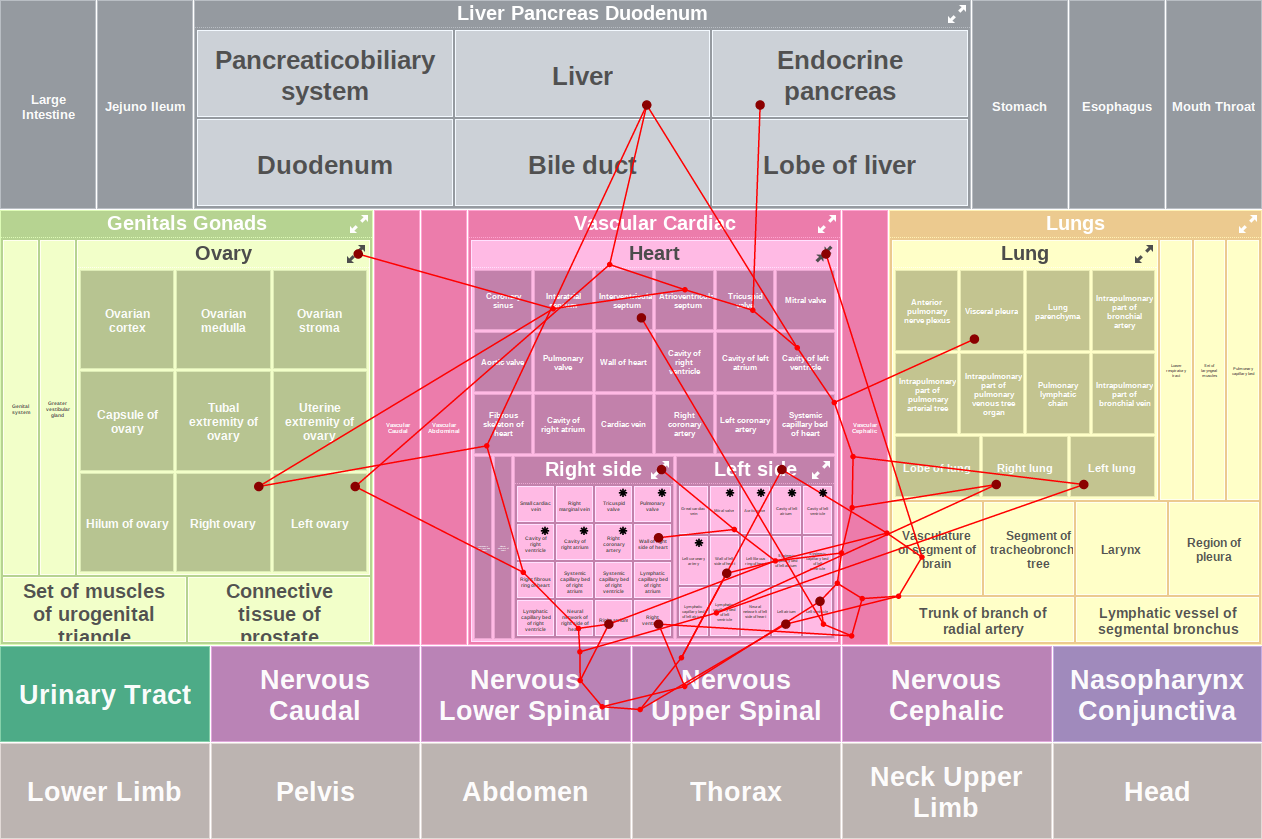
\includegraphics[width=5.8cm]{images/screenshot-bloodvessels.png}
    \label{fig:bloodvessels} % TODO: refer to this
  }%
  \subfigure[Arterial connections from left ventricle]{
    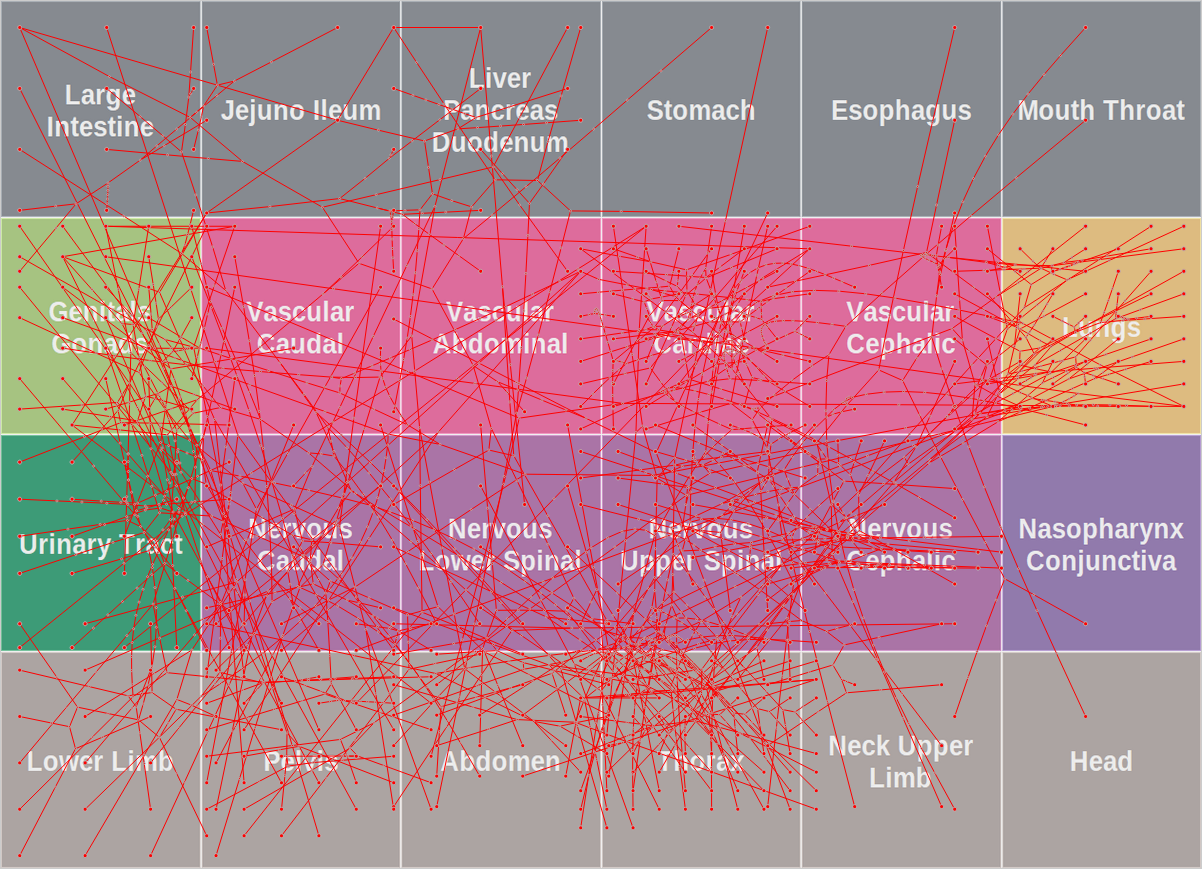
\includegraphics[width=5.8cm,height=3.855cm]{images/force-7101-new.png}
    \label{fig:force-7101}
  }\vskip-2mm
  \subfigure[Bundled paths from left ventricle]{
    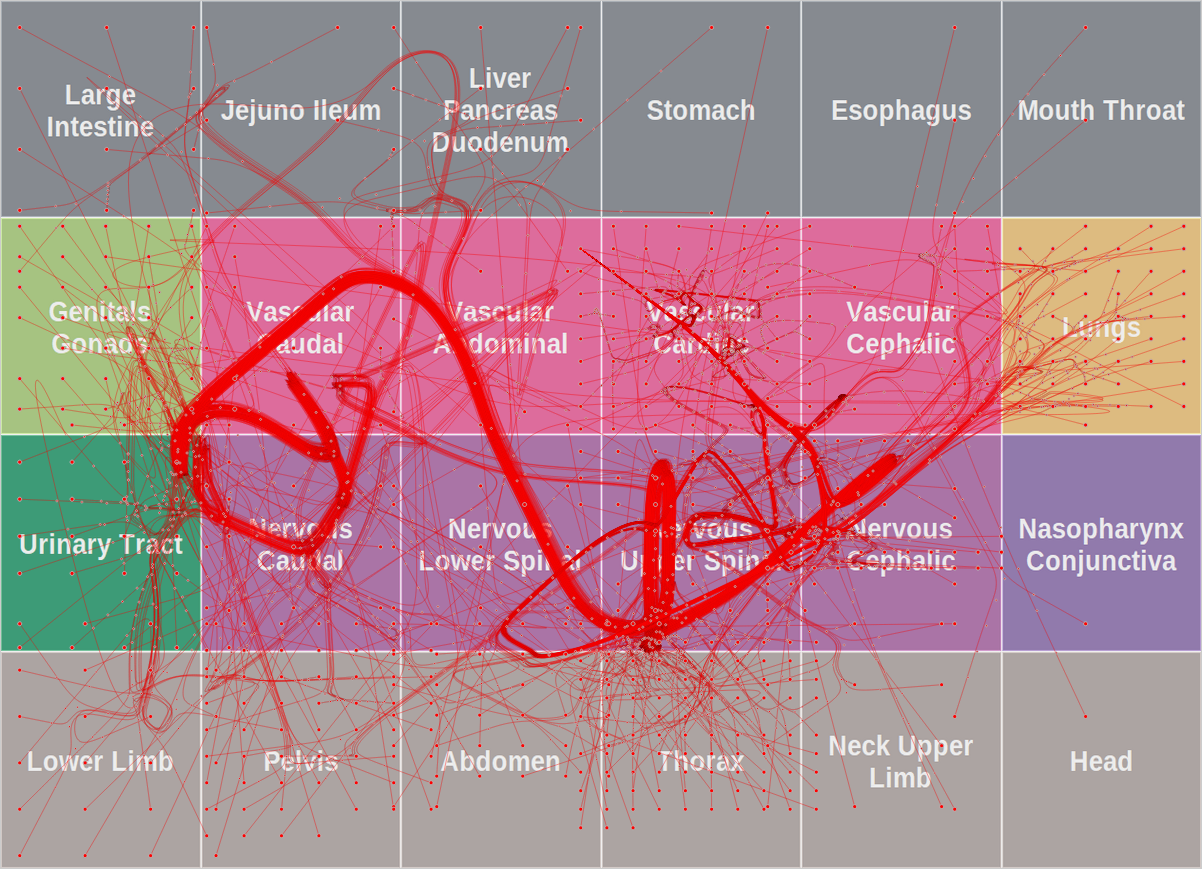
\includegraphics[width=5.8cm,height=3.855cm]{images/connections-7101-new.png}
    \label{fig:bundled-7101}
  }%
  \subfigure[Bundled paths to right atrium]{
    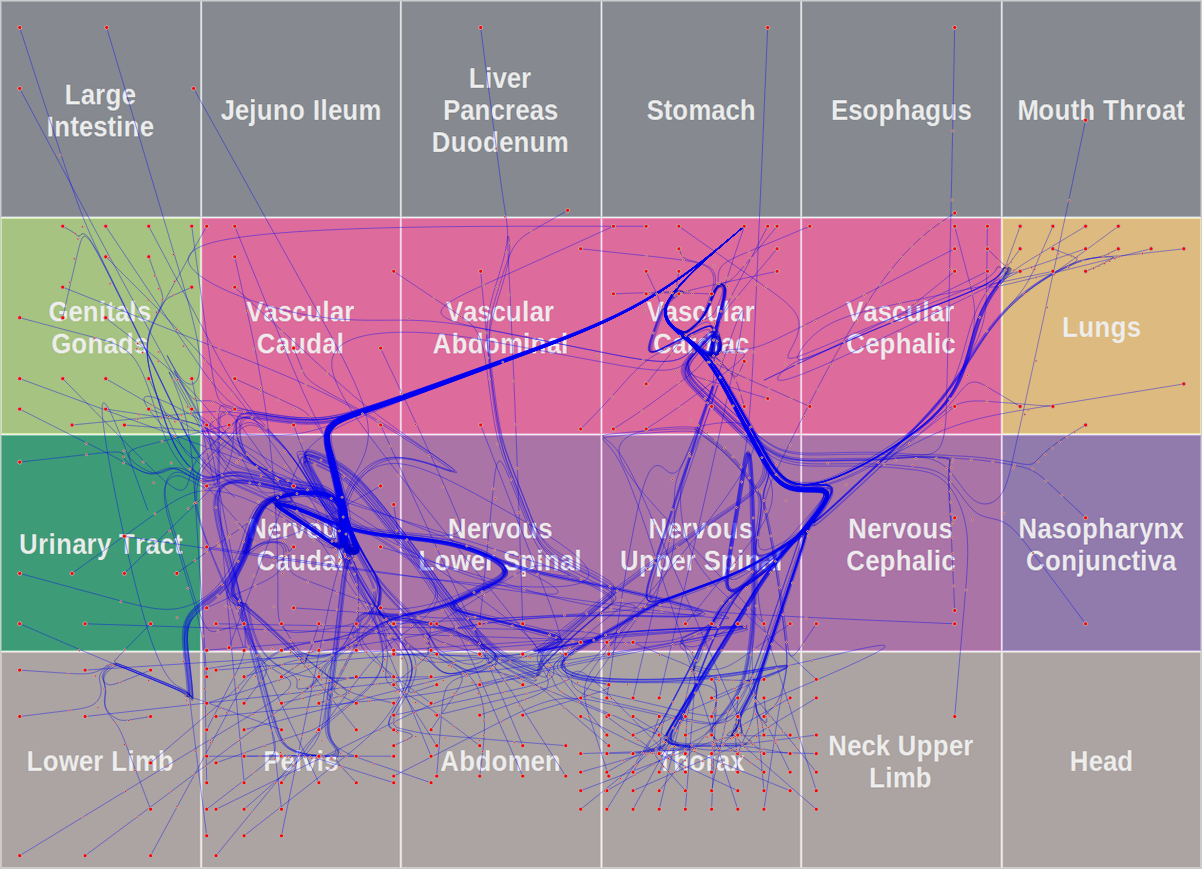
\includegraphics[width=5.8cm,height=3.855cm]{images/connections-7096b-new.png}
    \label{fig:bundled-7096}
  }\vskip1mm
  \caption{Cardiovascular system}
  \label{fig:vascular-connectivity}
\end{figure}

After a one-time pre-processing to import data from available external sources, we store connectivity data in a convenient format. A user can interact with and edit this data using our application.

One of the prime goals of the tool is to simplify the access and maintenance of biomedical taxonomies, including those concerned with physiological connectivity data. A user should be able to customize the way in which that data is represented. There is ongoing work on an implementation of the orthogonal connector visualization algorithm that would place edges into margins between tiles so that they will not obstruct the interaction with the tiles themselves.


%%%%%%%%%%%%%%%%%%%%%%%%%%%%%%%%%%%%%%%%%%%%%%%%%%%%%%%%%%%%%%%%%%%%%%%%%%%%%%%%%%%%%%%%%%
\section{Visualization of Models and Metadata} \label{sect:visualization2}               %
%%%%%%%%%%%%%%%%%%%%%%%%%%%%%%%%%%%%%%%%%%%%%%%%%%%%%%%%%%%%%%%%%%%%%%%%%%%%%%%%%%%%%%%%%%

The entities in the ApiNATOMY ontologies have various data associated with them, to which they are explicitly linked via semantic metadata annotations. This includes, for instance, static and dynamic 3D models of body organs and their subsystems.
To illustrate the application of ApiNATOMY in the management of semantic metadata and associated resources, we extract and display neuronal reconstructions and associated metadata from \url{http://neuromorpho.org}~\cite{Asc06}.
\Cref{fig:neuron-big} shows a sample neuron model associated with the neocortex (reached through``Nervous Cephalic'' $\rightarrow$ ``Region of cerebral cortex'' $\rightarrow$ ``Neocortex''). ApiNATOMY allows users to show multiple 3D objects together in their proper context. For example, \cref{fig:neuron-small} shows a screenshot of a circuit board with the ``Neocortex'' neuron, as well as 3D models of the ``Liver'' and ``Stomach''.

\begin{figure*}
\centering
  \subfigure[Neuron in the ``Neocortex'']{
    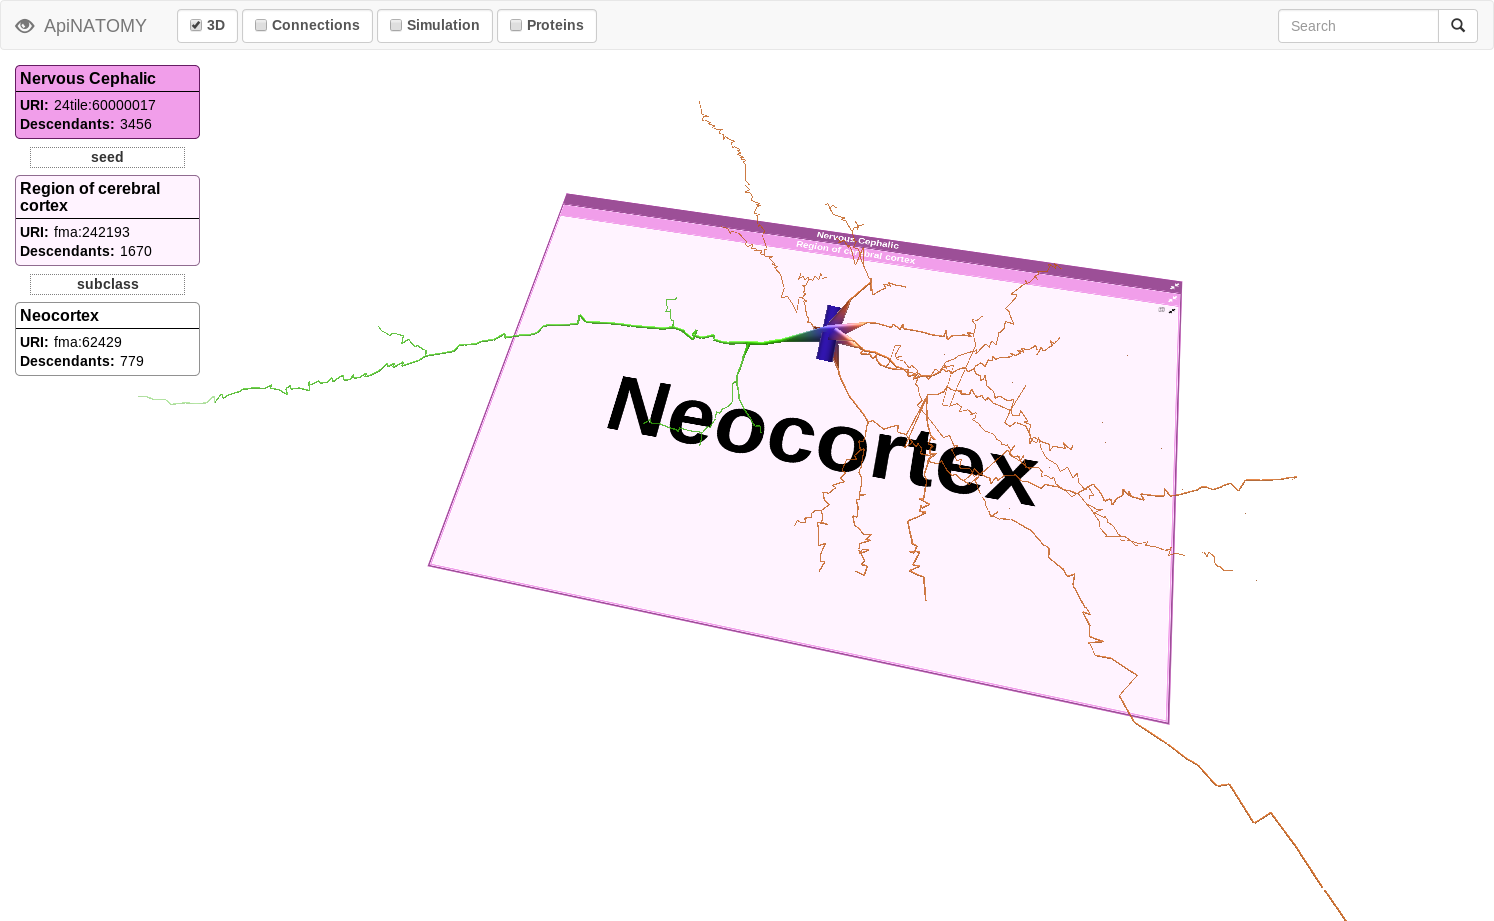
\includegraphics[width=5.4cm]{images/screenshot-neocortex-neuron.png}
    \label{fig:neuron-big}
  }
  \subfigure[Multiple 3D models in context]{
    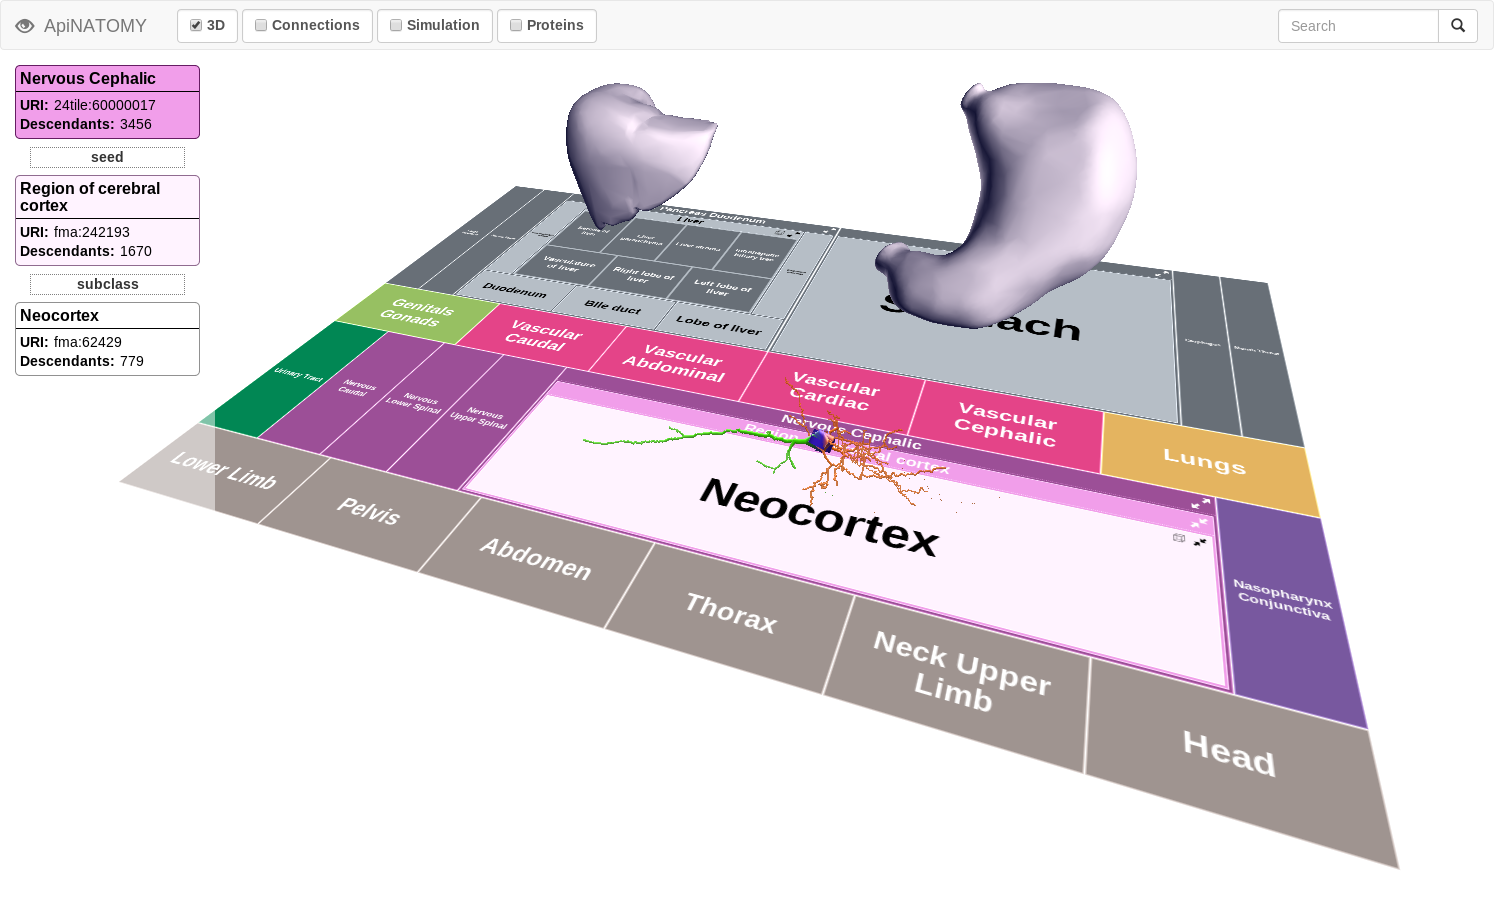
\includegraphics[width=5.4cm]{images/screenshot-3d-objects.png}
    \label{fig:neuron-small}
  }\vskip2mm
  \caption{Visualization of static 3D models}
  \label{fig:neurons}
\end{figure*}

ApiNATOMY also supports the visualization of protein- and drug-interaction networks (\cref{fig:protein}) that are represented as graphs on top of treemap tiles. We are in the process of acquiring and integrating relevant data from the Ensembl genomic database~\cite{Ensemble}. In Ensembl, gene models are annotated automatically using biological sequences data (e.g. protein, mRNA). We query this database to extract genes, transcripts, and translations with related protein features such as e.g., PFAM domains, and locate automatically-generated diagrams of proteins with FMA tiles to represent the anatomical location in which they are expressed. For ease of visualisation, protein diagrams show domain features built from different shapes and colors in a navigable 3D environment (\cref{fig:protein-3d}).

\begin{figure*}
\centering
%	\subfigure[Simulation control panel]{
%		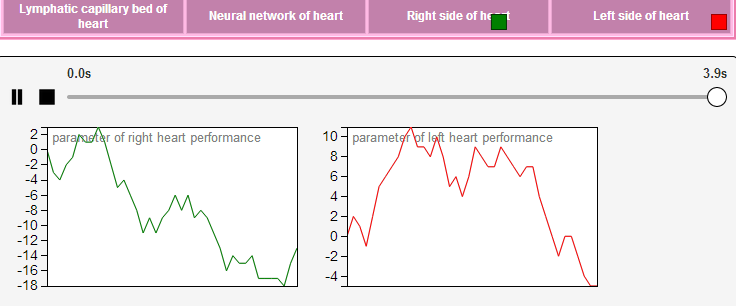
\includegraphics[width=5cm]{images/simulation.png}
%		\label{fig:panel}
%	}
	\subfigure[Protein interactions in 2D]{
		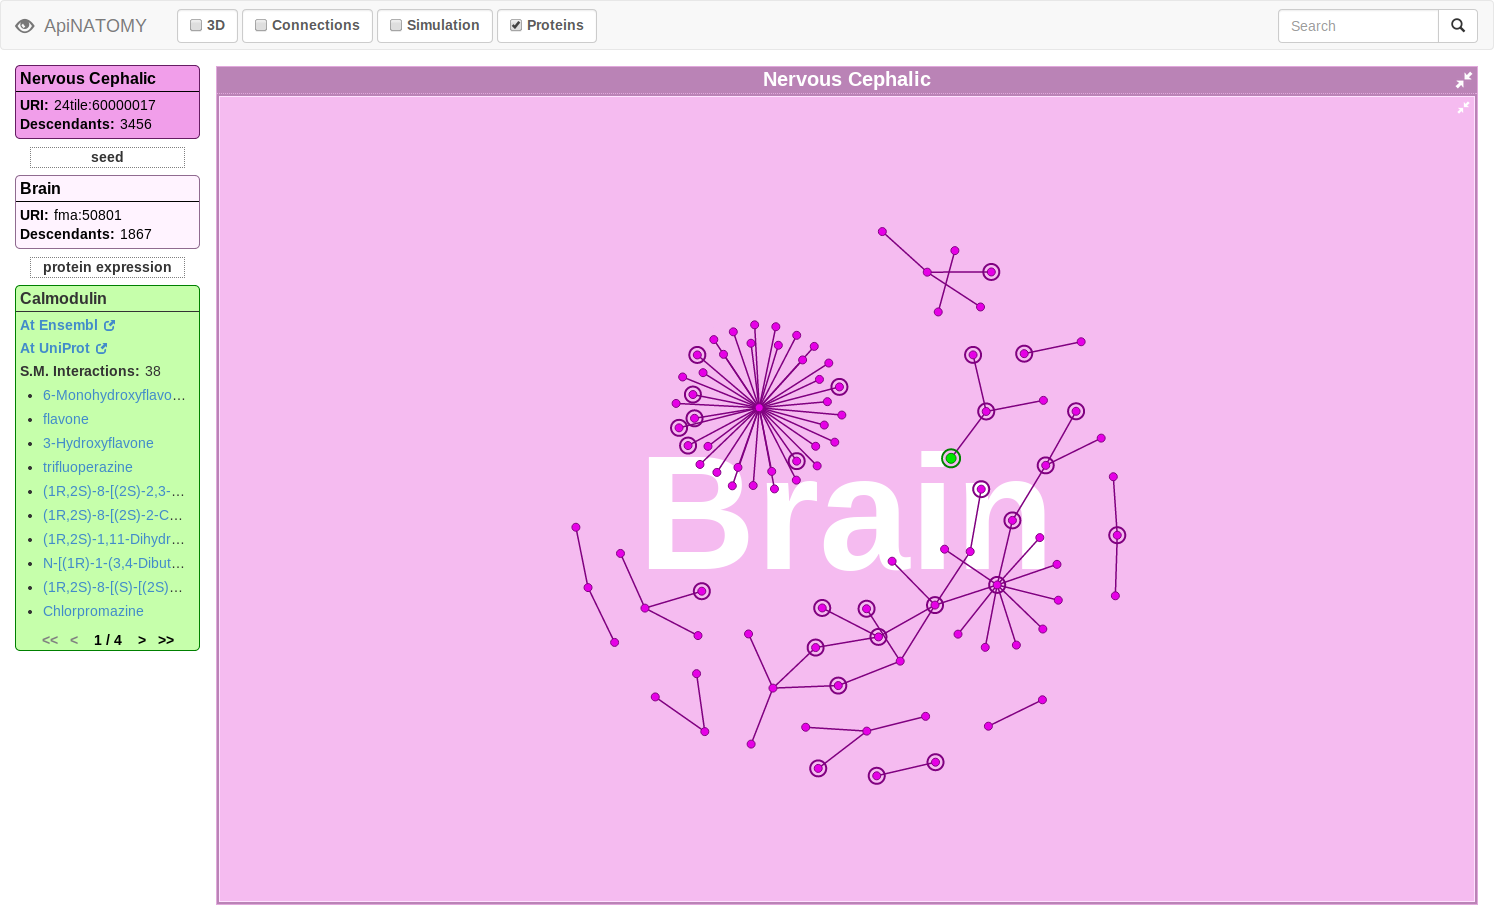
\includegraphics[width=5.4cm]{images/screenshot-proteins.png}
		\label{fig:protein}
	}
	\subfigure[Protein features in 3D]{
		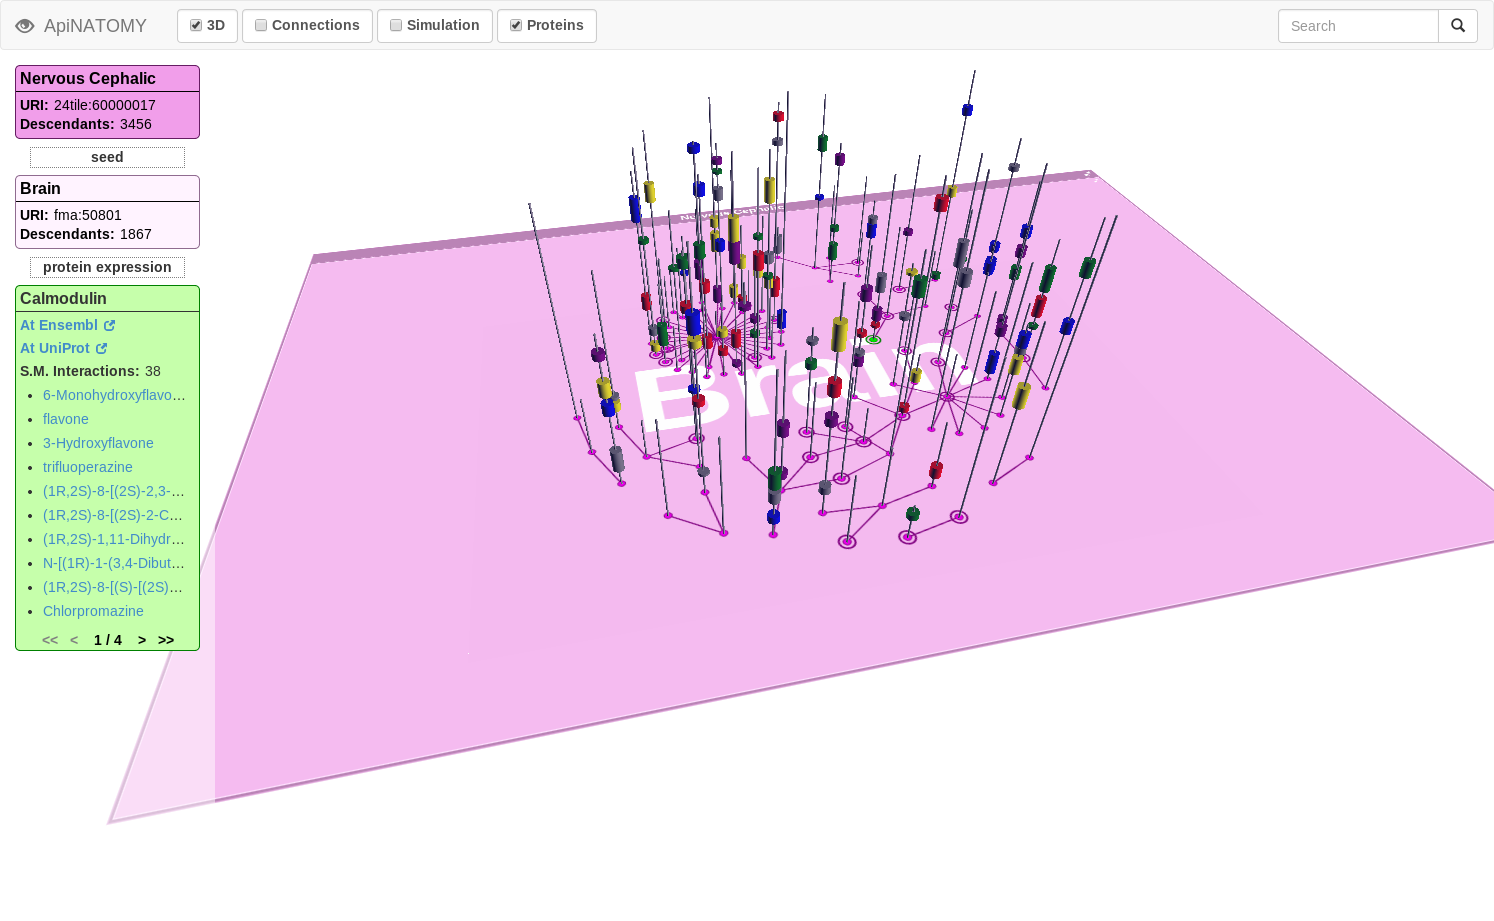
\includegraphics[width=5.4cm]{images/screenshot-proteins-3d.png}
		\label{fig:protein-3d}
	}
	\caption{Visualizing protein expression, protein interaction and protein features}
	\label{fig:proteins}
\end{figure*}
